\documentclass[12pt]{article}
\author{Alex Ho}
\title{AST5220 - Cosmology 2 \\ Milestone 1}
\usepackage{listings}
\usepackage{graphicx}
\usepackage{verbatim}
\usepackage{amsmath}
\usepackage{float}
\usepackage[utf8]{inputenc}
\usepackage{xcolor}
\usepackage{booktabs}
\usepackage{hyperref}
\usepackage{placeins}
\usepackage{parskip}
\setlength\parskip{\baselineskip}
\setlength\parindent{0pt}

\lstset{
language=Python,
basicstyle=\ttfamily,
otherkeywords={__init__},             
keywordstyle=\ttfamily\color{blue!90!black},
keywords=[2]{True,False},
keywordstyle={[2]\ttfamily\color{red!40!black}},
emph={MyClass,class, def},          
emphstyle=\ttfamily\color{red!83!black},    
stringstyle=\color{green!45!black},
showstringspaces=false,
commentstyle=\color{magenta},
breaklines=true,
tabsize=3,
moredelim=**[is][\color{blue}]{@}{@}
}

\begin{document}
\maketitle
The program, plots and the report can be found in the following Github page:

https://github.com/AHo94/AST5220\_Projects/tree/master/Project1
\subsection*{Mathematics}
We will be solving the first order differential equation given in (11) from the project sheet. First, we rewrite the equation from the dependence of the scale factor to a dependence the variable $x=\ln a$ or $a = e^x$. From this, one can rewrite the ordinary and scaled Hubble parameter (without taking neutrinos into account) as
\begin{align}
H(x) &= H_0 \sqrt{(\Omega_b + \Omega_m)e^{-3x} + \Omega_r e^{-4x} + \Omega_{\Lambda}} \label{eq:Hubble_param} \\
\mathcal{H}(x) &=e^{x}H(x) = H_0\sqrt{(\Omega_b + \Omega_m)e^{-x} + \Omega_re^{-2x} + \Omega_{\Lambda}e^{2x}}
\end{align}
The derivative of the scaled Hubble parameter, with respect to x, is then
\begin{align*}
\frac{d\mathcal{H}}{dx} = -\frac{H_0^2}{\mathcal{H}}\left( \frac{1}{2}(\Omega_b + \Omega_m)e^{-x} + \Omega_r e^{-2x}  -\Omega_{\Lambda}e^{2x}\right)
\end{align*}
The left-hand side of the differential equation can be written as
\begin{align}
\frac{d\eta}{da} = \frac{d\eta}{dx}\frac{dx}{da}
\end{align}
By differentiating $a=e^{x}$, we get
\begin{align}
\frac{dx}{da} = \left(\frac{da}{dx} \right)^{-1} = e^{-x}
\end{align}
The differential equation we have to solve is then
\begin{align}
\frac{d\eta}{dx} = \frac{c}{\mathcal{H}}
\label{eq:Differential_eq_eta}
\end{align}
In order to plot the relative densities (the $\Omega$s), we will first have to calculate the energy densities today, $\rho_{i,0}$, for a component $i$. Once this is calculated, the relative density of a component $i$, at an arbitrary time, is then
\begin{align}
\Omega_i = \frac{\rho_{i,0}}{\rho_{\text{crit}}}a^{-3(1+w)}
\end{align}
Where $\rho_{\text{crit}} = (3H(x)^2)/(8\pi G)$ is the critical density which depends on the Hubble parameter $H(x)$, given in \ref{eq:Hubble_param}. The parameter $w$ is the equation of state, and takes value $w=1$ for baryonic and dark matter, $w=1/3$ for radiation (and neutrinos) and $w=-1$ for dark energy.

\subsection*{Numerics}
The program is written in Python, with all essential codes written in one Python class. The constructor of the class initializes all the required arrays that we have used in the program. The constructor takes in two arguments. The argument \verb|savefile| shows all the plots if it takes the value 0 and saves the plots to a pdf file if it takes the value 1. 

The differential equation , given in \ref{eq:Differential_eq_eta}, was solved using the function \verb|odeint|, from the \verb|scipy.integrate| package. One thing to note is that this function only solves first order differential equations. In case we have second order differential equation(s), we would have to rewrite it to a first order differential equation. From this, we obtained an array of $\eta$, which is later used to interpolate other $\eta$ values for an arbitrary point.

The function \verb|Get_eta| takes in the calculated $\eta$, as well as the corresponding $x$ values, which will be used for the interpolation. The final three remaining arguments in the \verb|Get_eta| function determines start and end range of the new $x$ array and the number of interpolated points respectively. Inside this function, we first let \texttt{scipy.interpolate} determine the smoothness of the curve using the function \texttt{splrep}. We then define the range of the new $x$ variable, which is then used to give us the interpolated $\eta$ values, using the \texttt{splev} function.

The relative densities are calculated in the function \verb|Get_Omegas|. As described in the previous section, we will have to calculate, for each component, the energy density today, which is then used to calculate the relative density at an arbitrary time. The energy density today is a constant and can thus be pre-calculated, which will save us some computation time. The Hubble parameter in the critical density is simply called from the function \verb|Get_Hubble_param|.

Finally, we have the function \verb|Plot_results|, which uses \texttt{scipy}'s integration function to solve the differential equation, calls the \verb|Get_eta| function to interpolate, and plots our desired results. \verb|Plot_results| takes in one argument which indicates the number of interpolated points one wishes to have, and two optional arguments \verb|x_start| and \verb|x_end| which indicates the starting and ending segment of the interpolation respectively. The optional arguments, by default, are set to the start and end of recombination respectively.

When the program plots the interpolated points of the conformal time, it will also make a plot that is zoomed in on the interpolated segment. All plots can be found in the next section with some extra details in the caption. The program can be found at the end of the report.

\newpage
\subsection*{Plots}
\begin{figure}[h]
\centering
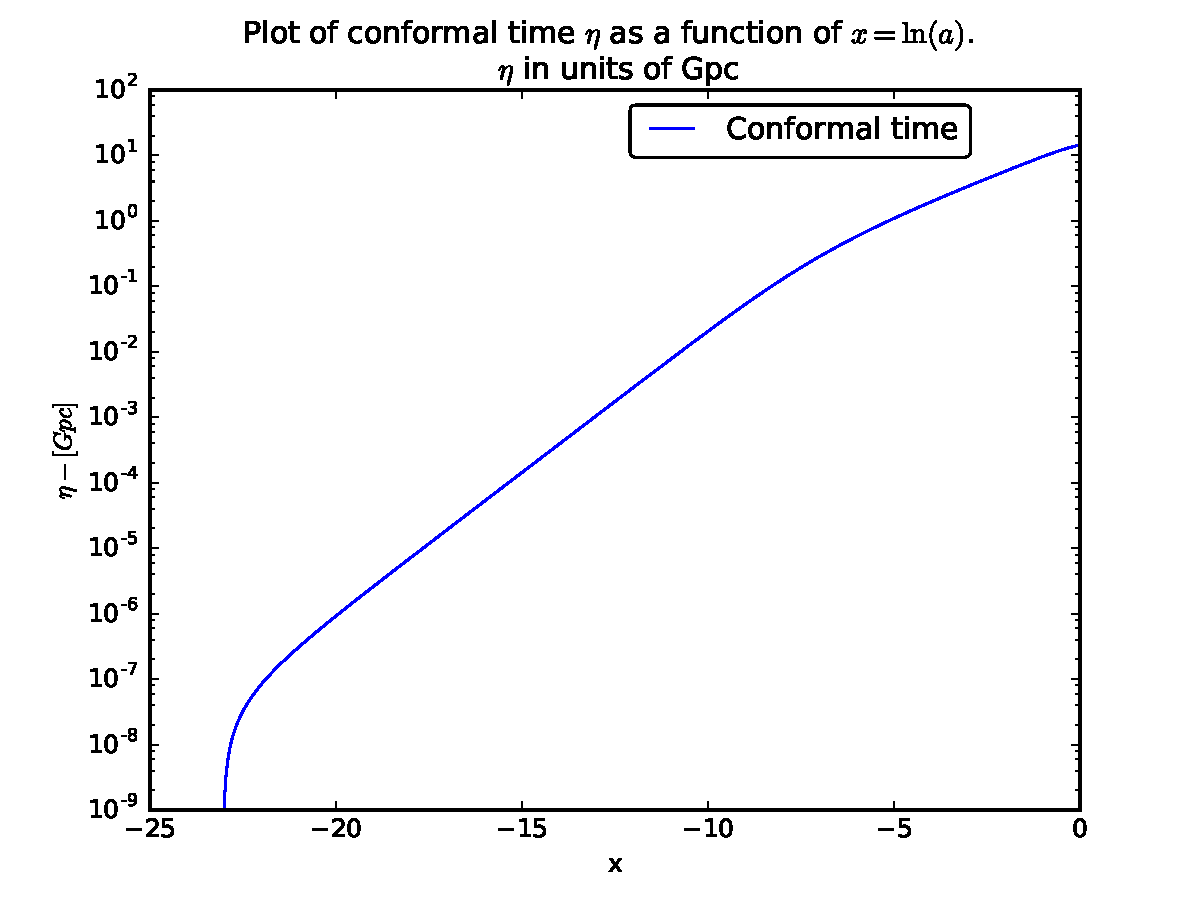
\includegraphics[width=\linewidth]{Plots/ConformalTime_SanityCheck.pdf}
\caption{A plot of the conformal time as a function of $x=\ln (a)$. This plot serves as a sanity check whether the program is correct or wrong. As we see, the conformal time is roughly $14-15 Gpc$ today, which is what we expect.}
\label{fig:Conformal_time}
\end{figure}

\begin{figure}[h]
\centering
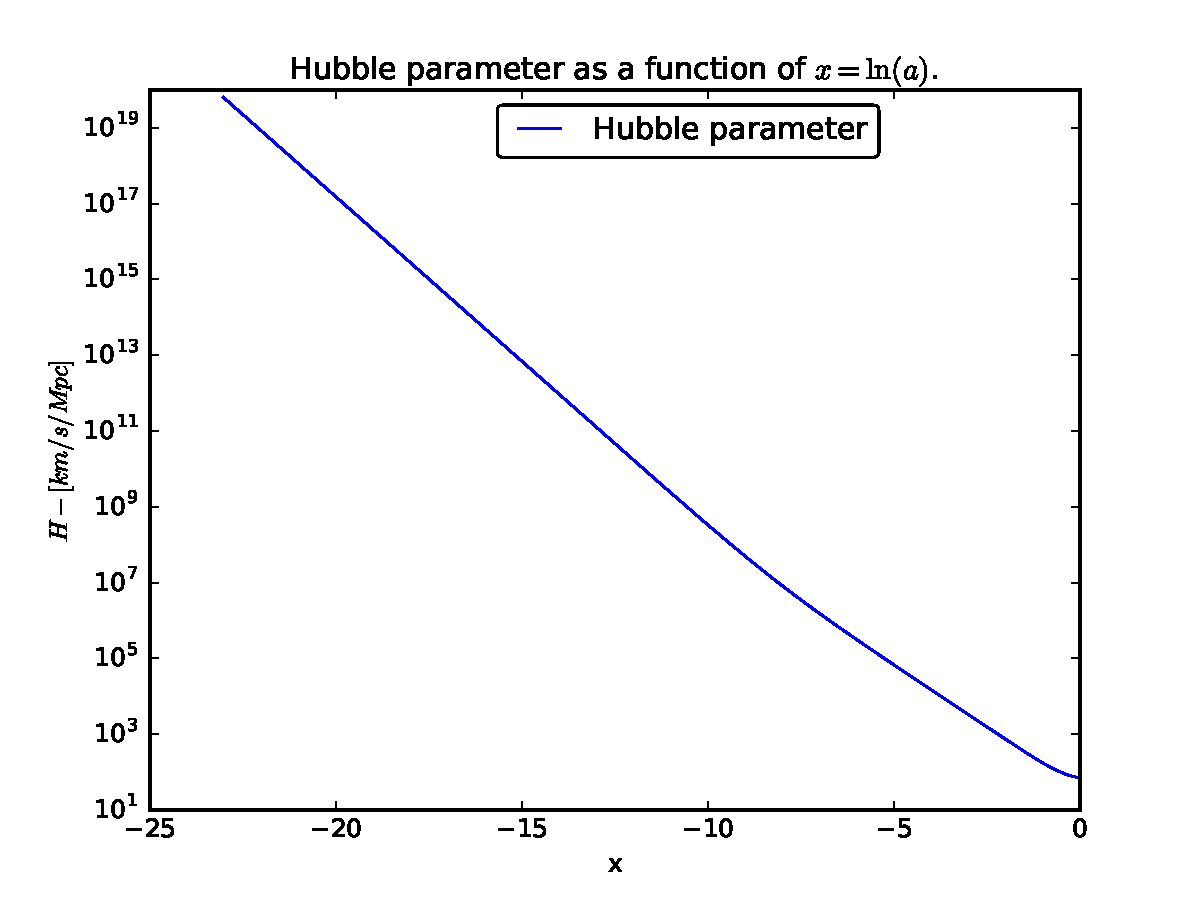
\includegraphics[width=0.8\linewidth]{Plots/Hubble_parameter.pdf}
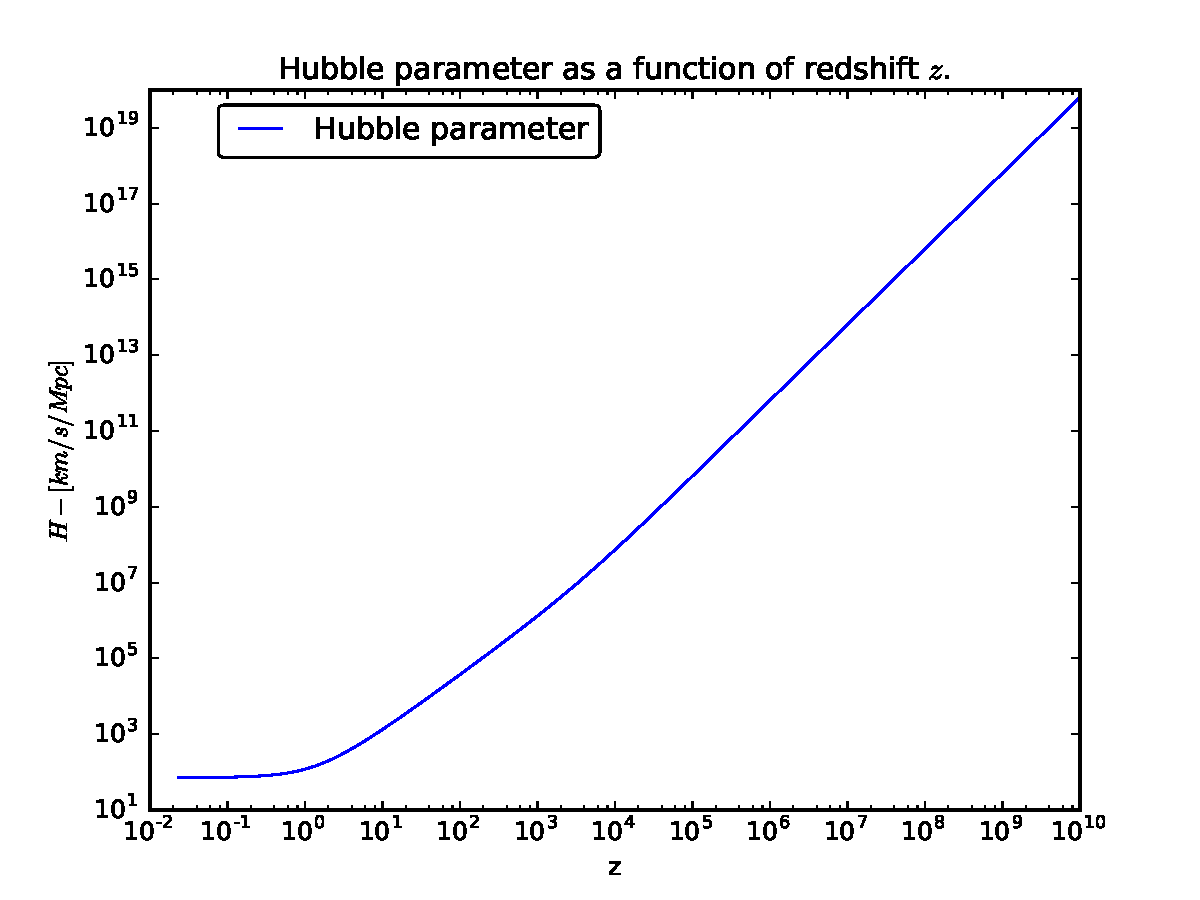
\includegraphics[width=0.8\linewidth]{Plots/Hubble_parameter_redshift.pdf}
\caption{Plots of the Hubble parameter as a function of $x=\ln(a)$ (top image) and redshift $z$ (bottom image). Both plots shows that the Hubble parameter is roughly 70 km/s/Mpc today, and increases as we go back in time (corresponds to larger $z$ and smaller $x$).}
\label{fig:Hubble_parameter_plot}
\end{figure}

%Plot of the Hubble parameter as a function of $x=\ln(a)$. Tt may be difficult to see, but the Hubble parameter is $70$km/s/Mpc today, which is what we would expect.

%\begin{figure}[h]
%\centering
%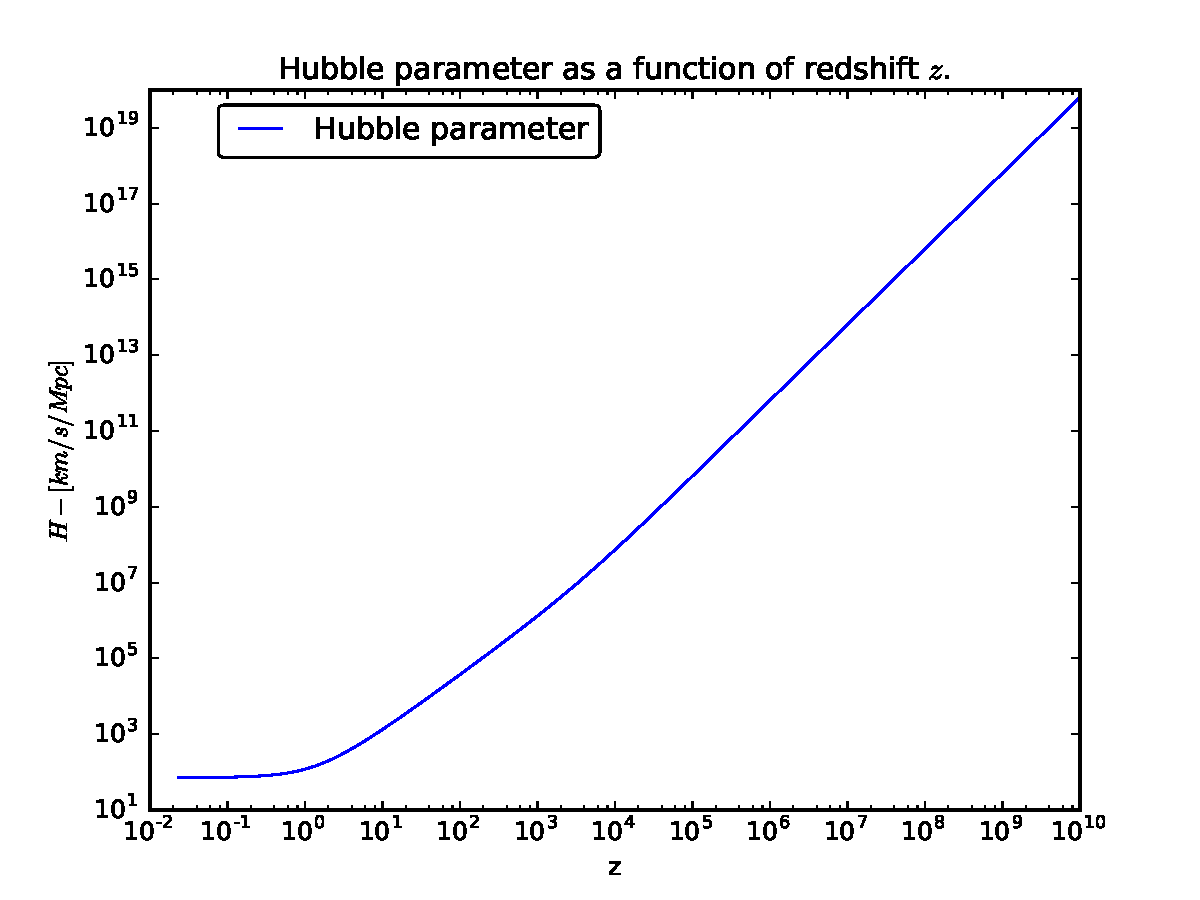
\includegraphics[width=\linewidth]{Plots/Hubble_parameter_redshift.pdf}
%\caption{Hubble parameter as a function of redshift $z = 1/a - 1$. The results are exactly the same as the previous plot of the Hubble parameter. Again, the Hubble parameter today, $z=0$ is roughly $70$km/s/Mpc, and it increases as we go further back in time (increased redshift).}
%\end{figure}

\begin{figure}[hbtp]
\centering
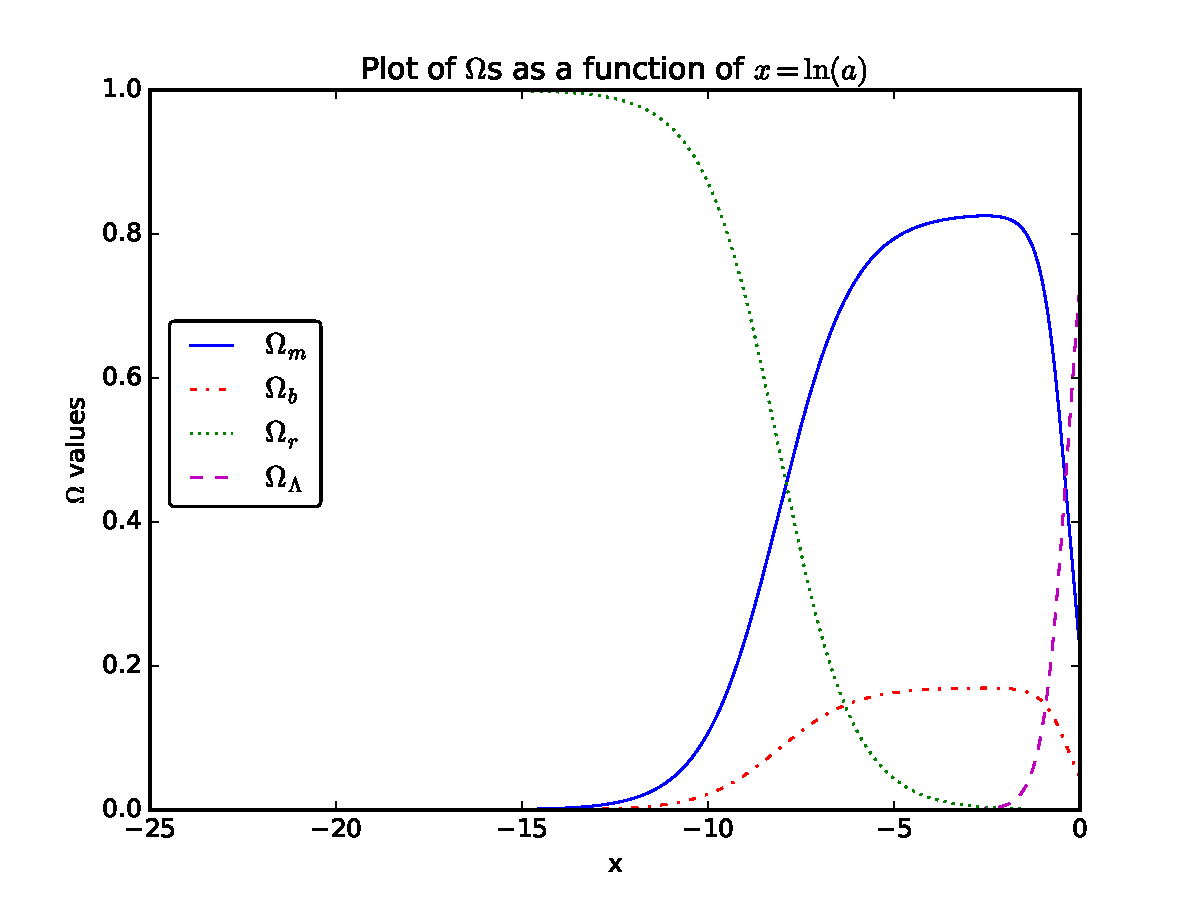
\includegraphics[width=\linewidth]{Plots/Omegas.pdf}
\caption{A plot of the relative densities $\Omega$ as a function of $x=\ln(a)$. We see that radiation (dotted) was the dominant component in the early times of the universe. As time passes, matter (line) becomes dominant, with dark matter (dash-dot) being the most dominant component. Finally, near the recent times the component of dark energy (dashed) increases rapidly.}
\end{figure}

\begin{figure}[h]
\centering
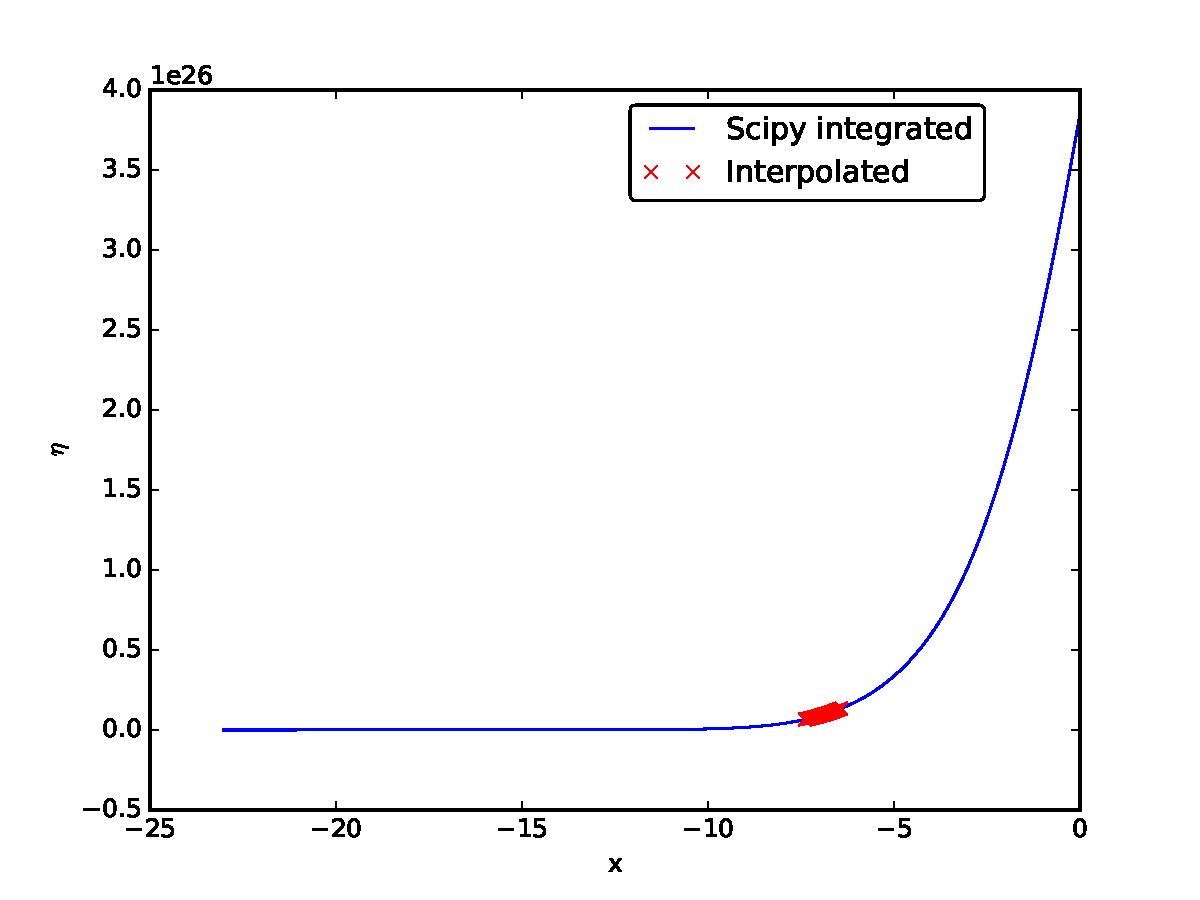
\includegraphics[width=0.82\textwidth]{Plots/Interpolated_Example.pdf}
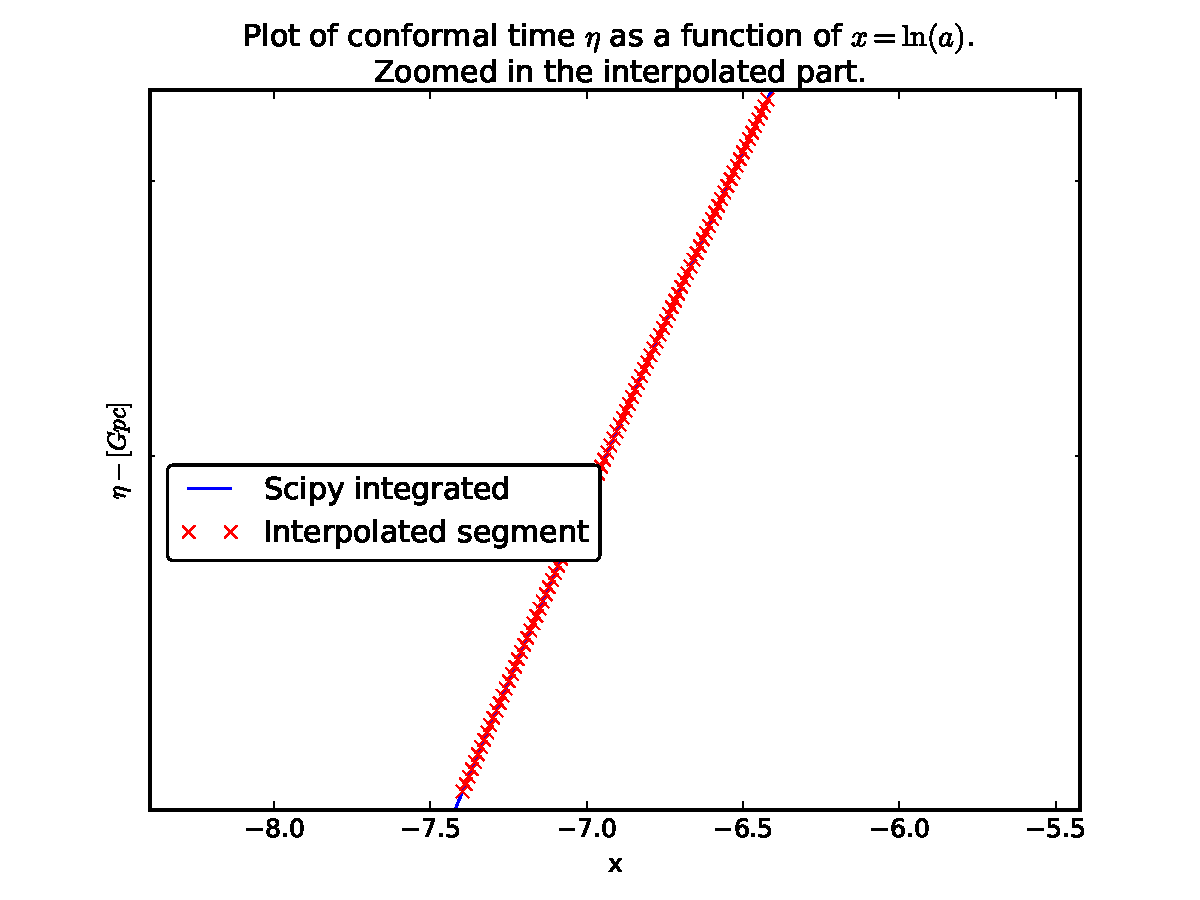
\includegraphics[width=0.82\textwidth]{Plots/Interpolated_Example_zoomed.pdf}
\caption{Top image shows an example of the interpolated points. The example shows interpolated points in the time when recombination started to the end of recombination. The bottom image is zoomed in to the interpolated section.}
\label{fig:Interpolated_point}
\end{figure}


\FloatBarrier
\subsection*{The program}
\begin{lstlisting}
import numpy as np
import matplotlib.pyplot as plt
from scipy import interpolate
from scipy import integrate

# Global constants
# Units
eV = 1.60217647e-19
Mpc = 3.08568025e22

# Cosmological parameters
Omega_b = 0.046
Omega_m = 0.224
Omega_r = 8.3e-5
Omega_nu = 0.0
Omega_lambda = 1.0 - Omega_m - Omega_b - Omega_r - Omega_nu
T_0 = 2.725
n_s = 1.0
A_s = 1.0
h0 = 0.7
H_0 = h0*100.0*1e3/Mpc

# General constants
c = 2.99792458e8
epsilon_0 = 13.605698*eV
m_e = 9.10938188e-31
m_H = 1.673534e-27
sigma_T = 6.652462e-29
G_grav = 6.67258e-11
rho_c0 = (3.0*H_0**2)/(8*np.pi*G_grav)
alpha = 7.29735308e-3
hbar = 1.05457148e-34
k_b = 1.3806503e-23

# Density Parameters today
rho_m0 = Omega_m*rho_c0
rho_b0 = Omega_b*rho_c0
rho_r0 = Omega_r*rho_c0
rho_lambda0 = Omega_lambda*rho_c0


class time_mod():
	def __init__(self, savefig):
		self.savefig = savefig		# If savefig = 0, plots the data. If savefig = 1, saves the plots in a pdf

		if savefig != 0 and savefig != 1:
			print 'Current value of savefig = ', savefig
			raise ValueError('Argument savefig not properly set. Try savefig = 1 (saves as pdf) or savefig = 0 (do not save as pdf)')

		self.n1 = 200
		self.n2 = 300
		self.n_t = self.n1 + self.n2

		self.z_start_rec = 1630.4
		self.z_end_rec = 614.2
		self.z_0 = 0.0
		self.x_start_rec = -np.log(1.0 + self.z_start_rec)
		self.x_end_rec = -np.log(1.0 + self.z_end_rec)
		self.x_0 = 0.0
		self.a_start_rec = 1.0/(1.0 + self.z_start_rec)
		self.a_end_rec = 1.0/(1.0 + self.z_end_rec)

		# Used for the x-values for the conformal time
		self.n_eta = 1000
		self.a_init = 1e-10
		self.x_eta_init = np.log(self.a_init)
		self.x_eta_end = 0

		# Set up grid, these are currently unused
		x_t_rec = np.linspace(self.x_start_rec, self.x_end_rec, self.n1)
		x_t_today = np.linspace(self.x_end_rec, self.x_0, self.n2)
		a_t_rec = np.linspace(self.a_start_rec, self.a_end_rec, self.n1)
		a_t_today = np.linspace(self.a_end_rec, 1, self.n2)
		# Merging the arrays into one
		self.x_t = np.concatenate([x_t_rec, x_t_today])
		self.a_t = np.concatenate([a_t_rec, a_t_today])

		# Set up grid of x-values for the integrated eta
		self.x_eta = np.linspace(self.x_eta_init, self.x_eta_end, self.n_eta)	# X-values for the conformal time

	def Get_Hubble_param(self, x):
		""" Function returns the Hubble parameter for a given x """
		return H_0*np.sqrt((Omega_b + Omega_m)*np.exp(-3*x) + Omega_r*np.exp(-4*x) + Omega_lambda)

	def Get_Hubble_prime(self, x):
		""" Function returns the scaled Hubble parameter for a given x value. See report """
		return H_0*np.sqrt((Omega_b + Omega_m)*np.exp(-x) + Omega_r*np.exp(-2*x) + Omega_lambda*np.exp(2*x))

	def Get_Hubble_prime_derivative(self, x):
		""" Function returns the derivative of the scaled Hubble parameter. See report """
		return -H_0**2*(0.5*(Omega_b + Omega_m)*np.exp(-x) + Omega_r*np.exp(-2*x) - Omega_lambda*np.exp(2*x))/(Get_Hubble_prime(x))

	def Get_Omegas(self, x):
		""" 
		Calculates the omegas as a function of redshift
		Will first have to calculate the energy densities today, which is then used to calculate the energy density
		for an arbitrary time. See report
		"""
		H = self.Get_Hubble_param(x)		# Hubble parameter for an arbitrary time
		rho_c = (3*H**2)/(8*np.pi*G_grav)	# Critical density for an arbitrary time
		Omega_m_z = rho_m0*np.exp(-3*x)/rho_c
		Omega_b_z = rho_b0*np.exp(-3*x)/rho_c
		Omega_r_z = rho_r0*np.exp(-4*x)/rho_c
		Omega_lambda_z = rho_lambda0/rho_c

		return Omega_m_z, Omega_b_z, Omega_r_z, Omega_lambda_z

	def Diff_eq(self, y, x_init):
		""" Returns the right hand side of the differential equation """
		dEtada = c/(self.Get_Hubble_prime(x_init))
		return dEtada

	def Get_eta(self, x_values, eta_values, x_start, x_end, n_points):
		""" Cubic spline interpolation, zeroth derivative. Returns interpolated eta for a given range of x-values """
		Temp_interp = interpolate.splrep(x_values, eta_values)
		x_new = np.linspace(x_start, x_end, n_points)
		eta_new = interpolate.splev(x_new, Temp_interp, der=0)
		return x_new, eta_new

	def Spline_DoubleDerivative(self, x_values, eta_values):
		""" 
		Evaluates the second derivatives at each grid point.
		Boundaries for the double derivatives are zero, using the so called natural spline 
		"""
		Temp_interp = interpolate.splrep(x_values, eta_values)
		etaDoubleDer = interpolate.splev(x_values, Temp_interp, der=2)
		etaDoubleDer[0] = 0
		etaDoubleDer[-1] = 0
		return etaDoubleDer

	def Get_Index_Interpolation(self, X_init, X_end):
		""" 
		Finds the array index/component of x for a given x-value
		This is specifically used to zoom into the interpolated segment
		"""
		EtaIndex1 = (np.abs(self.x_eta - X_init)).argmin()
		EtaIndex2 = (np.abs(self.x_eta - X_end)).argmin()
		if EtaIndex1-1 <= 0:
			EtaIndex1 = 0
		else:
			EtaIndex1 -= 1

		if EtaIndex2+1 >= self.n_eta:
			EtaIndex2 = self.n_eta-1
		else:
			EtaIndex2 += 1

		return EtaIndex1, EtaIndex2

	def Plot_results(self, n_interp_points, x_start = -np.log(1.0 + 1630.4), x_end = -np.log(1.0 + 614.2)):
		""" Solves and plots the results """
		self.ScipyEta = integrate.odeint(self.Diff_eq, self.x_eta_init, self.x_eta)
		x_eta_new, eta_new = self.Get_eta(self.x_eta, self.ScipyEta, x_start, x_end, n_interp_points)

		fig1 = plt.figure()
		ax1 = plt.subplot(111)
		ax1.semilogy(self.x_eta, self.ScipyEta/(Mpc*1e3), 'b-', label='Conformal time')
		plt.xlabel('x')
		plt.ylabel('$\eta - [Gpc]$')
		ax1.legend(loc='upper left', bbox_to_anchor=(0.5,1), ncol=1, fancybox=True)
		plt.title('Plot of conformal time $\eta$ as a function of $x = \ln (a)$. \n $\eta$ in units of Gpc')

		fig2 = plt.figure()
		ax2 = plt.subplot(111)
		ax2.semilogy(self.x_eta, self.Get_Hubble_param(self.x_eta)*Mpc/1e3, label='Hubble parameter')
		plt.xlabel('x')
		plt.ylabel(r'$H - [km/s/Mpc]$')
		plt.title('Hubble parameter as a function of $x = \ln (a)$.')
		ax2.legend(loc='upper right', bbox_to_anchor=(0.8,1), ncol=1, fancybox=True)

		fig3 = plt.figure()
		ax3 = plt.subplot(111)
		z_eta = 1/(np.exp(self.x_eta)) - 1 		# Convert x-values to redshift values, with z = 1/a - 1
		ax3.loglog(z_eta, self.Get_Hubble_param(np.log(1/(1+z_eta)))*Mpc/1e3, label='Hubble parameter')
		plt.xlabel('z')
		plt.ylabel(r'$H - [km/s/Mpc]$')
		plt.title('Hubble parameter as a function of redshift $z$.')
		ax3.legend(loc='upper right', bbox_to_anchor=(0.5,1), ncol=1, fancybox=True)
		
		Om_m, Om_b, Om_r, Om_lambda = self.Get_Omegas(self.x_eta)
		fig4 = plt.figure()
		ax4 = plt.subplot(111)
		plt.hold("on")
		ax4.plot(self.x_eta, Om_m, 'b-', label='$\Omega_m$')
		ax4.plot(self.x_eta, Om_b, 'r-.', label='$\Omega_b$')
		ax4.plot(self.x_eta, Om_r, 'g:', label='$\Omega_r$')
		ax4.plot(self.x_eta, Om_lambda, 'm--', label='$\Omega_{\Lambda}$')
		plt.xlabel('x')
		plt.ylabel('$\Omega$ values')
		plt.title('Plot of $\Omega$s as a function of $x=\ln(a)$')
		ax4.legend(loc='upper right', bbox_to_anchor=(0.2,0.7), ncol=1, fancybox=True)

		fig5 = plt.figure()
		ax5 = plt.subplot(111)
		plt.hold("on")
		ax5.semilogy(self.x_eta, self.ScipyEta/(Mpc*1e3), 'b-', label='Scipy integrated')
		ax5.semilogy(x_eta_new, eta_new/(Mpc*1e3), 'xr', label='Interpolated segment')
		plt.xlabel('x')
		plt.ylabel('$\eta - [Gpc]$')
		ax5.legend(loc='upper left', bbox_to_anchor=(0.1,1), ncol=1, fancybox=True)
		plt.title('Plot of conformal time $\eta$ as a function of $x = \ln (a)$')
		
		fig6 = plt.figure()
		ax6 = plt.subplot(111)
		plt.hold("on")		
		ax6.semilogy(self.x_eta, self.ScipyEta/(Mpc*1e3), 'b-', label='Scipy integrated')
		ax6.plot(x_eta_new, eta_new/(Mpc*1e3), 'xr', label='Interpolated segment')
		EtaIndex1, EtaIndex2 = self.Get_Index_Interpolation(x_start, x_end)
		plt.axis([x_start-1, x_end+1, self.ScipyEta[EtaIndex1]/(Mpc*1e3), self.ScipyEta[EtaIndex2]/(Mpc*1e3)])
		plt.xlabel('x')
		plt.ylabel('$\eta - [Gpc]$')
		ax6.legend(loc='upper right', bbox_to_anchor=(0.5,0.5), ncol=1, fancybox=True)
		plt.title('Plot of conformal time $\eta$ as a function of $x = \ln (a)$. \n Zoomed in the interpolated part.')

		if self.savefig == 1:
			fig1.savefig('../Plots/ConformalTime_SanityCheck.pdf')
			fig2.savefig('../Plots/Hubble_parameter.pdf')
			fig3.savefig('../Plots/Hubble_parameter_redshift.pdf')
			fig4.savefig('../plots/Omegas.pdf')
			fig5.savefig('../Plots/Interpolated_Example.pdf')
			fig6.savefig('../Plots/Interpolated_Example_zoomed.pdf')
			
		else:
			plt.show()

solver = time_mod(savefig=1)
solver.Plot_results(100)
\end{lstlisting}
\end{document}